\documentclass{article}
\usepackage{amsmath}
\usepackage{graphicx}

\begin{document}
\section{Reflection and Transmission on a Simple Boundary at Normal Incidence}
    \begin{figure}
        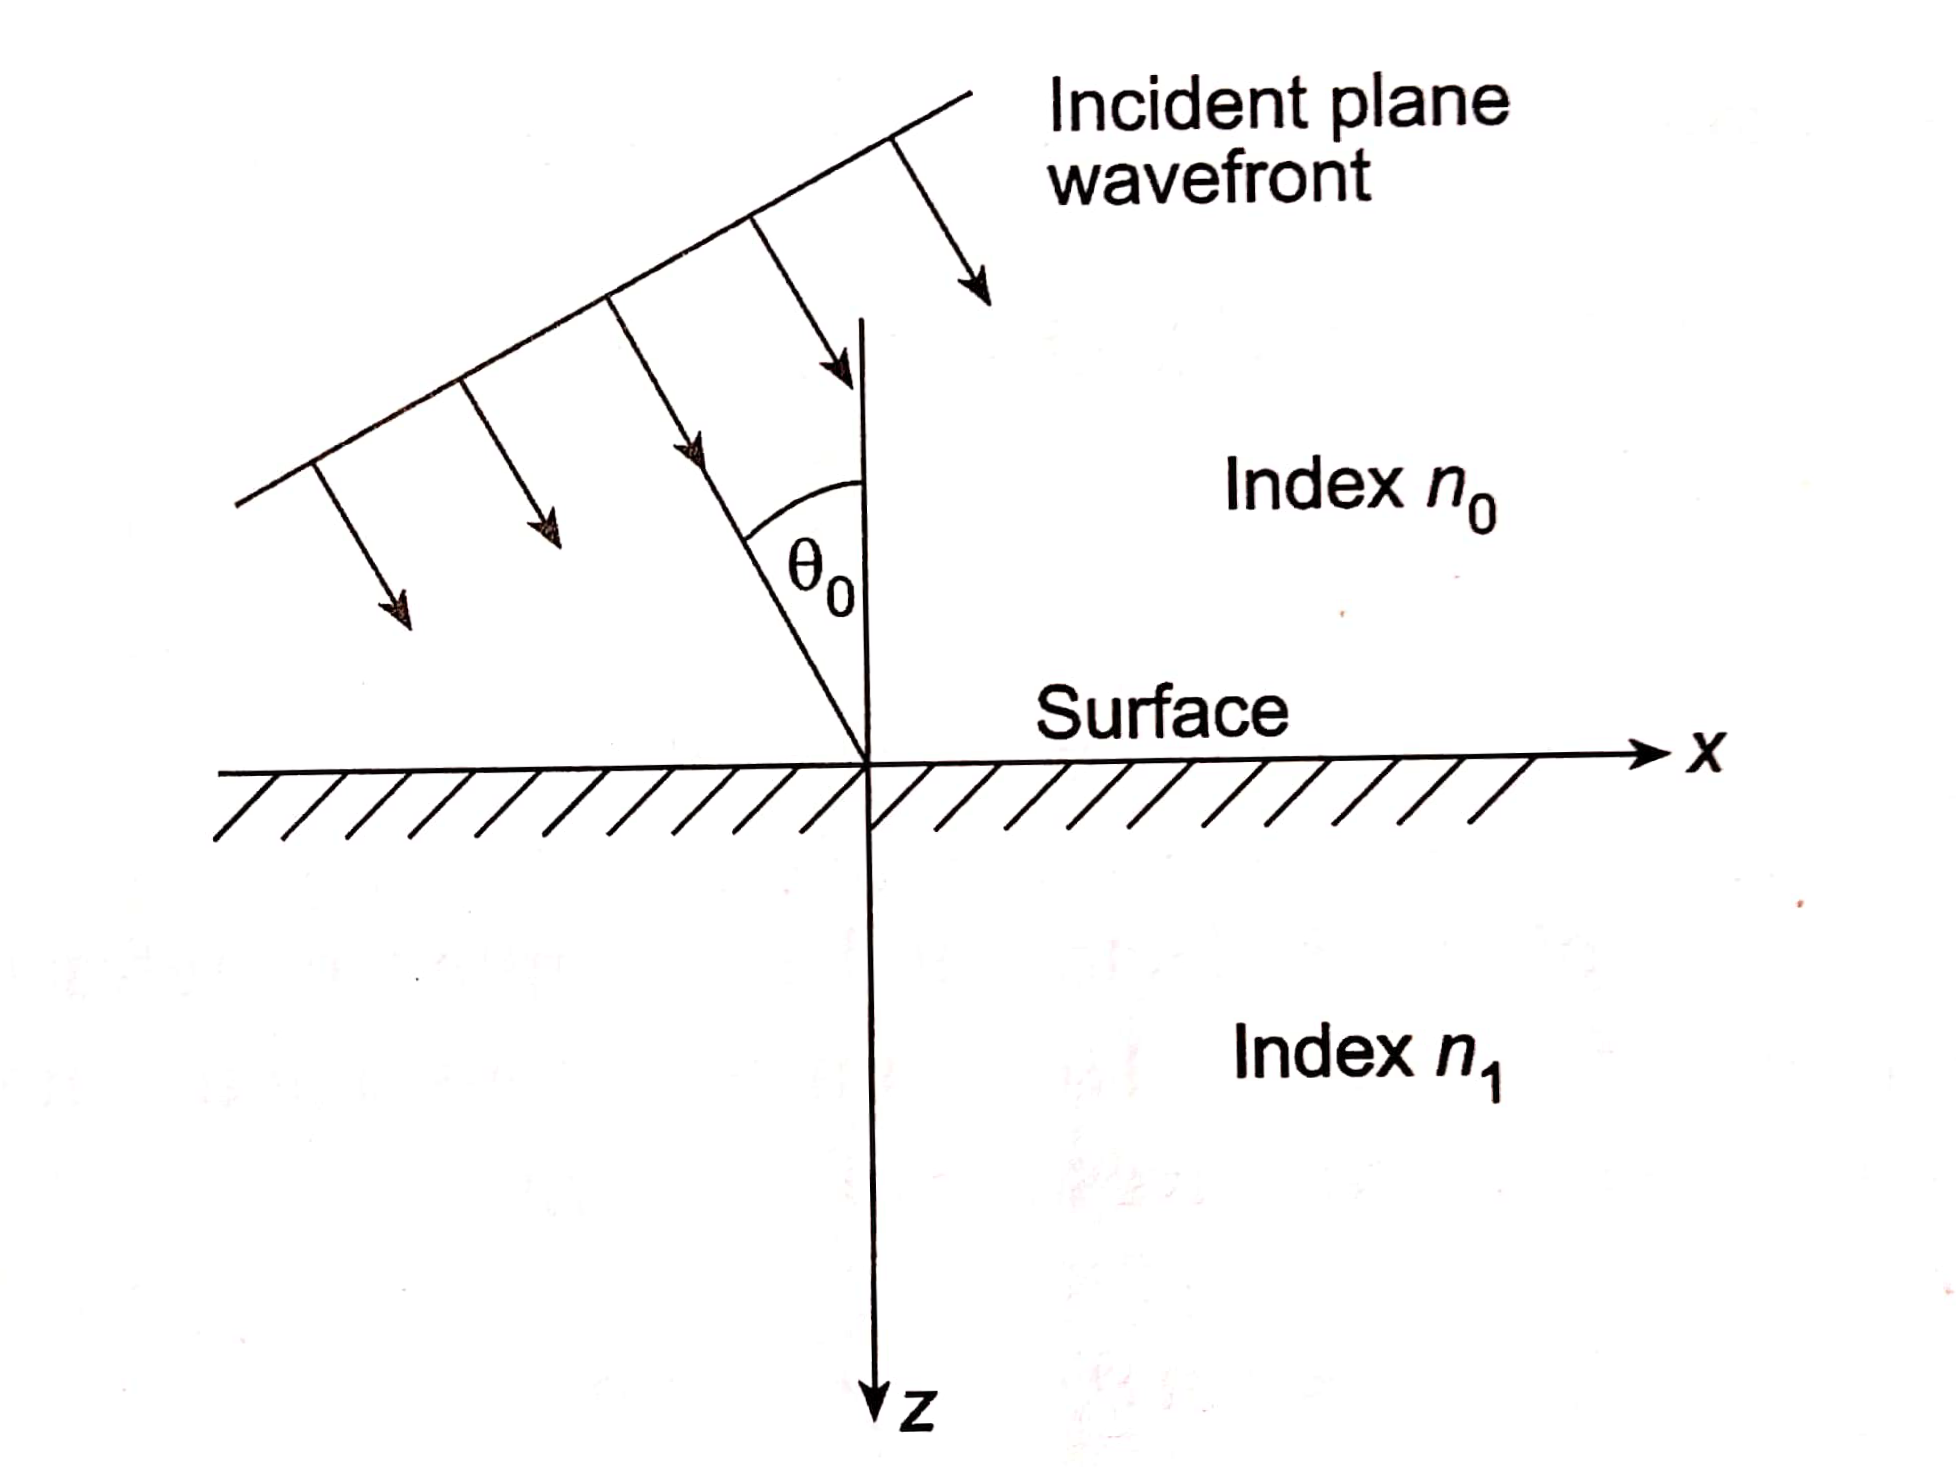
\includegraphics[width=\linewidth]{simple_boundary.png}
        \caption{Simple Boundary}
        \label{fig:simp}
    \end{figure}
    For an electromagnetic wave incident on a surface from index of refraction $n_0$ to $n_1$ at an angle $\theta_0$, the phase factors are given by
    \begin{align}
        &\text{Incident Wave} & &\mathrm{exp}\left\{ i [\omega t - (2\pi n_0 / \lambda)(x \sin \theta_0 - z \cos \theta_0)]\right\} \\
        &\text{Reflected Wave} & &\mathrm{exp}\left\{ i [\omega t - (2\pi n_0 / \lambda)(\alpha_r x + \beta_r y + \gamma_r z)]\right\} \\
        &\text{Transmitted Wave} & &\mathrm{exp}\left\{ i [\omega t - (2\pi n_1 / \lambda)(\alpha_t x + \beta_t y + \gamma_t z)]\right\}
    \end{align}
    This situation is schematically shown in Figure \ref{fig:simp}

    Let us temporarily consider light normally incident on the boundary. The electric field will be aligned along the positive x-direction, requiring the the magnetic field to be aligned along the positive y-axis. We apply the boundary conditions:
    \begin{enumerate}
        \item Electric field vector continuous across boundary
        \begin{equation}
            E_i + E_r = E_t
        \end{equation} 
        \item Magnetic field vector continuous across boundary
        \begin{equation}
            H_i - H_r = H_t
            \label{eq:magcont}
        \end{equation}
    \end{enumerate}
    Figure \ref{fig:norm} pictorially shows these conditions.

    \begin{figure}
        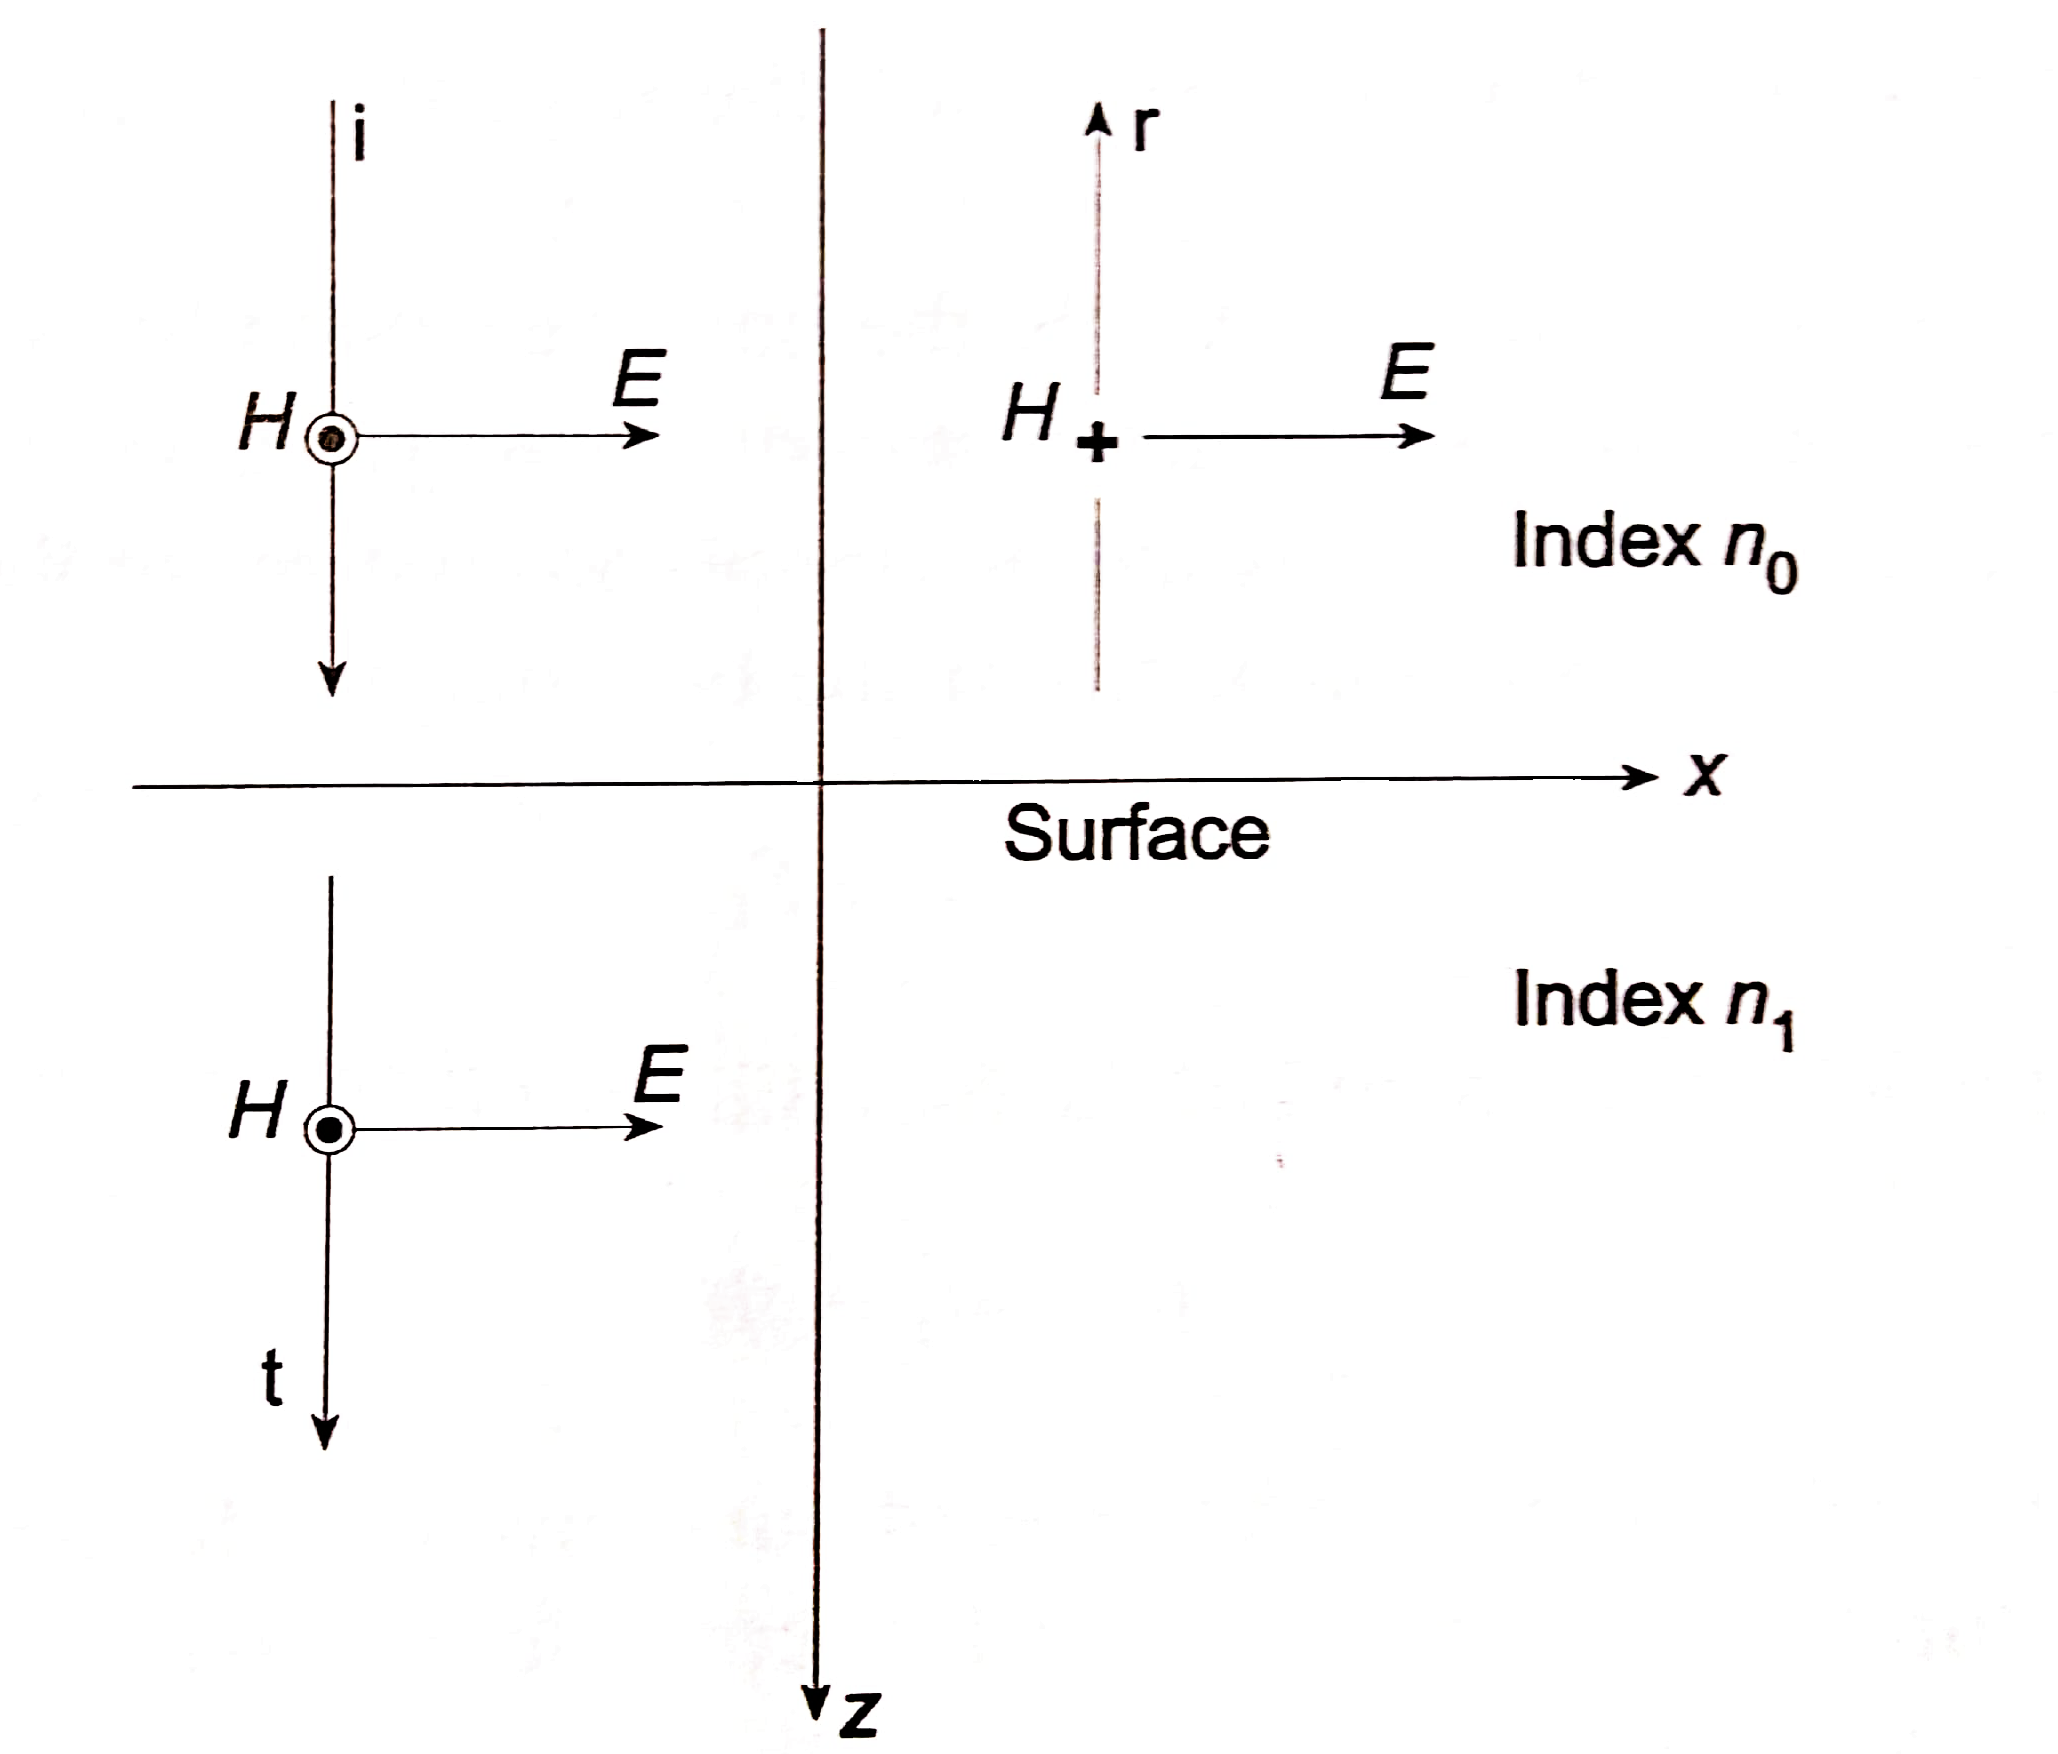
\includegraphics[width=\linewidth]{simple_boundary_normal.png}
        \caption{Light Normally incident on surface with electric and magnetic vectors shown}
        \label{fig:norm}
    \end{figure}

    Using the characteristic admittance, $y$, of each layer, Equation \ref{eq:magcont} can be expressed as

    \begin{equation}
        y_0 E_i - y_0 E_r = y_1 E_t \label{eq:admit}
    \end{equation}

    We can then compute the reflection coefficient $\rho$ and the transmission coefficient $\tau$
    \begin{align}
        \rho &= \frac{E_r}{E_i} = \frac{y_0 - y_1}{y_0 + y_1} = \frac{n_0 - n_1}{n_0 + n_1} \\
        \tau &= \frac{E_t}{E_i} = \frac{2 y_0}{y_0 + y_1} = \frac{2 n_0}{n_0+n_1}
    \end{align}
    Where the last equality comes about since in the optical regime
    $$ y = n y_{\mathrm{vaccuum}} $$

    And finally, we compute the transmittance $T$ and reflectance $R$ by
    \begin{align}
        T &= \frac{y_1}{y_0}\tau^2 = \frac{4 n_0 n_1}{(n_0 + n_1)^2} \label{eq:trans} \\
        R &= \rho^2 = \left(\frac{n_0 - n_1}{n_0 + n_1}\right)^2 \label{eq:reflec}
    \end{align}

    As expected for a non-absorbing medium $$ T + R = 1 $$

\section{Reflection and Transmission at Oblique Incidence}
    To extend this analysis to oblique incidence, we introduce the tilted optical admittance $\eta$ which connects the components of the electric and magnetic fields parallel to the boundary
    \begin{equation}
        \eta = \frac{H^{\parallel}}{E^{\parallel}}
    \end{equation}
    Using this tilted admittance, the transmission and reflection coefficients can be computed the same way they are computed in equations \ref{eq:trans} and \ref{eq:reflec}.

    From here, we will drop the $\parallel$ symbol, and $E$ and $H$ will be understood to mean $E^\parallel$ and $H^\parallel$ respectively, unless otherwise noted.

    It is worthy to note that to calculating $\eta$ depends on the polarization of incident light. In the case of s and p-polarization, the tilted admittances become
    \begin{align}
        \eta_p &= y/\cos \theta \\
        \eta_s &= y \cos \theta
    \end{align}
    Also of note is that this analysis can be readily extended to absorbing media if $\theta$ is allowed to be complex.

\section{Reflection of a Thin Film}
    We turn our attention to the geometry seen in Figure \ref{fig:film}. We first consider the tangential components of the electric and magnetic fields at boundary b, while introducing the notation $+$ referring to the positive-travelling wave and $-$ referring to waves traveling in the opposite direction.
    \begin{align}
        E_b &= E_{1b}^+ + E_{1b}^- \\
        H_b &= \eta_1 E_{1b}^+ - \eta_1 E_{1b}^-    
    \end{align}
    \begin{figure}
        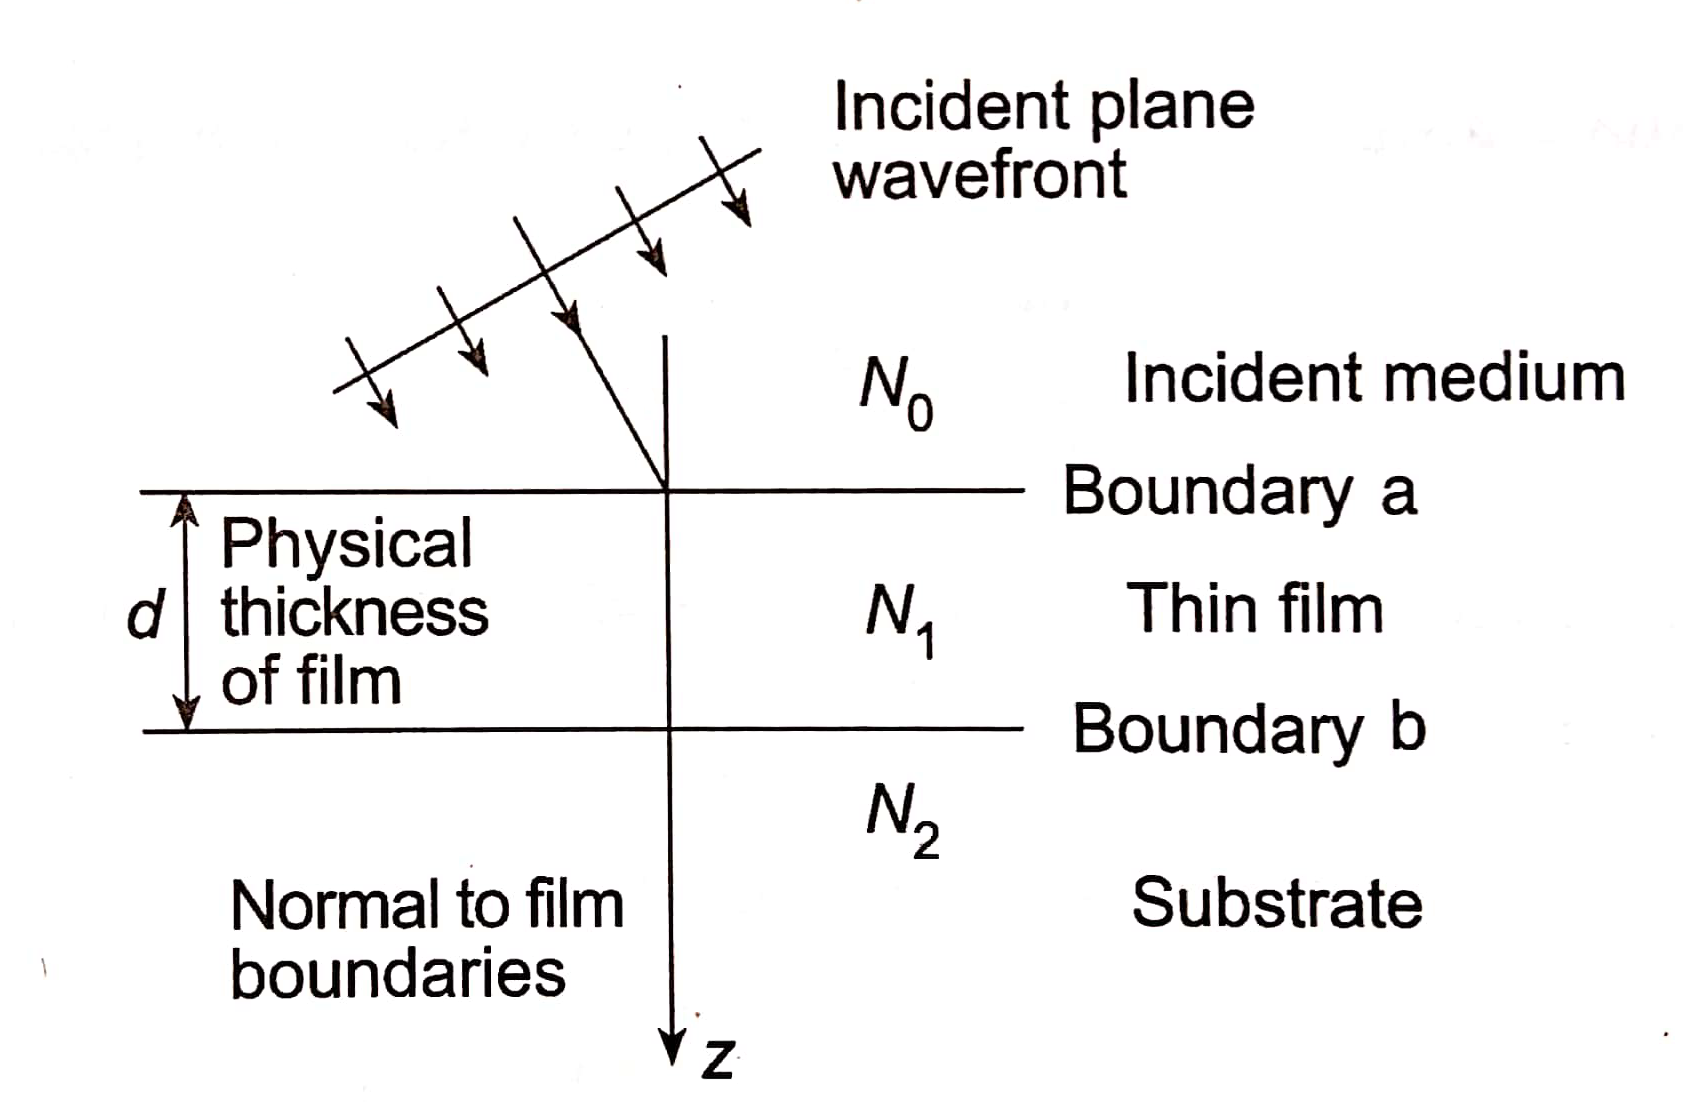
\includegraphics[width=\linewidth]{thin_film.png}
        \caption{Plane wave incident on a thin film}
        \label{fig:film}
    \end{figure}
    We can find the fields at the interface at $a$ by considering the phase difference at the same time, across the change in the $z$ coordinate by $-d$. We say that the positive going wave will be multiplied by $e^{i \delta}$ while the negative going wave will be multiplied by $e^{-i \delta}$ where
    \begin{equation}
        \delta = 2 \pi N_1 d \cos \theta_1 / \lambda    
    \end{equation}
    $N$ is the complex analogue to the refractive index $n$ and is given by $$N = n - ik $$ where $k$ is the extinction coefficient. $k$ is related to the absorption coefficient $\alpha$ by 
    \begin{equation}
        \alpha = \frac{4 \pi k}{\lambda}
    \end{equation}
    
    With these tools, we can relate $E_a$ and $H_a$ to $E_b$ and $H_b$ by the matrix equation
    \begin{equation}
        \label{eq:charmatrix}
        \begin{bmatrix}
            E_a \\
            H_a
        \end{bmatrix}
        =
        \begin{bmatrix}
            \cos \delta & (i \sin \delta)/\eta_1 \\
            i \eta_1 \sin \delta & \cos \delta
        \end{bmatrix}
        \begin{bmatrix}
            E_b \\
            H_b
        \end{bmatrix}        
    \end{equation}
    
    It will be convenient to normalize this equation
    \begin{equation}
        \begin{bmatrix}
            E_a/E_b \\
            H_a/E_b
        \end{bmatrix}
        =
        \begin{bmatrix}
            B \\
            C
        \end{bmatrix}
        =
        \begin{bmatrix}
            \cos \delta & (i \sin \delta)/\eta_1 \\
            i \eta_1 \sin \delta & \cos \delta
        \end{bmatrix}
        \begin{bmatrix}
            1 \\
            \eta_2
        \end{bmatrix}        
    \end{equation}
    The optical admittance of the assembly can be defined in an analogous way to what was used to write Equation \ref{eq:admit}
    \begin{equation}
        Y = \frac{H_a}{E_a} 
    \end{equation}
    and therefore
    \begin{equation}
        Y = \frac{C}{B} \label{eq:filmadmit}
    \end{equation}
    The reflectance of the thin film can then be written as
    \begin{equation}
        R = \left(\frac{\eta_0 - Y}{\eta_0 + Y}\right)\left(\frac{\eta_0 - Y}{\eta_0 + Y}\right)^* \label{eq:filmreflec}
    \end{equation}
    \begin{equation*}
        \begin{bmatrix}
            \cos \delta & (i \sin \delta)/\eta_1 \\
            i \eta_1 \sin \delta & \cos \delta
        \end{bmatrix}
    \end{equation*}
    is known as the \emph{characteristic matrix} of the film.   

\section{Reflectance of an Assembly of Thin Films}
    \begin{figure}
        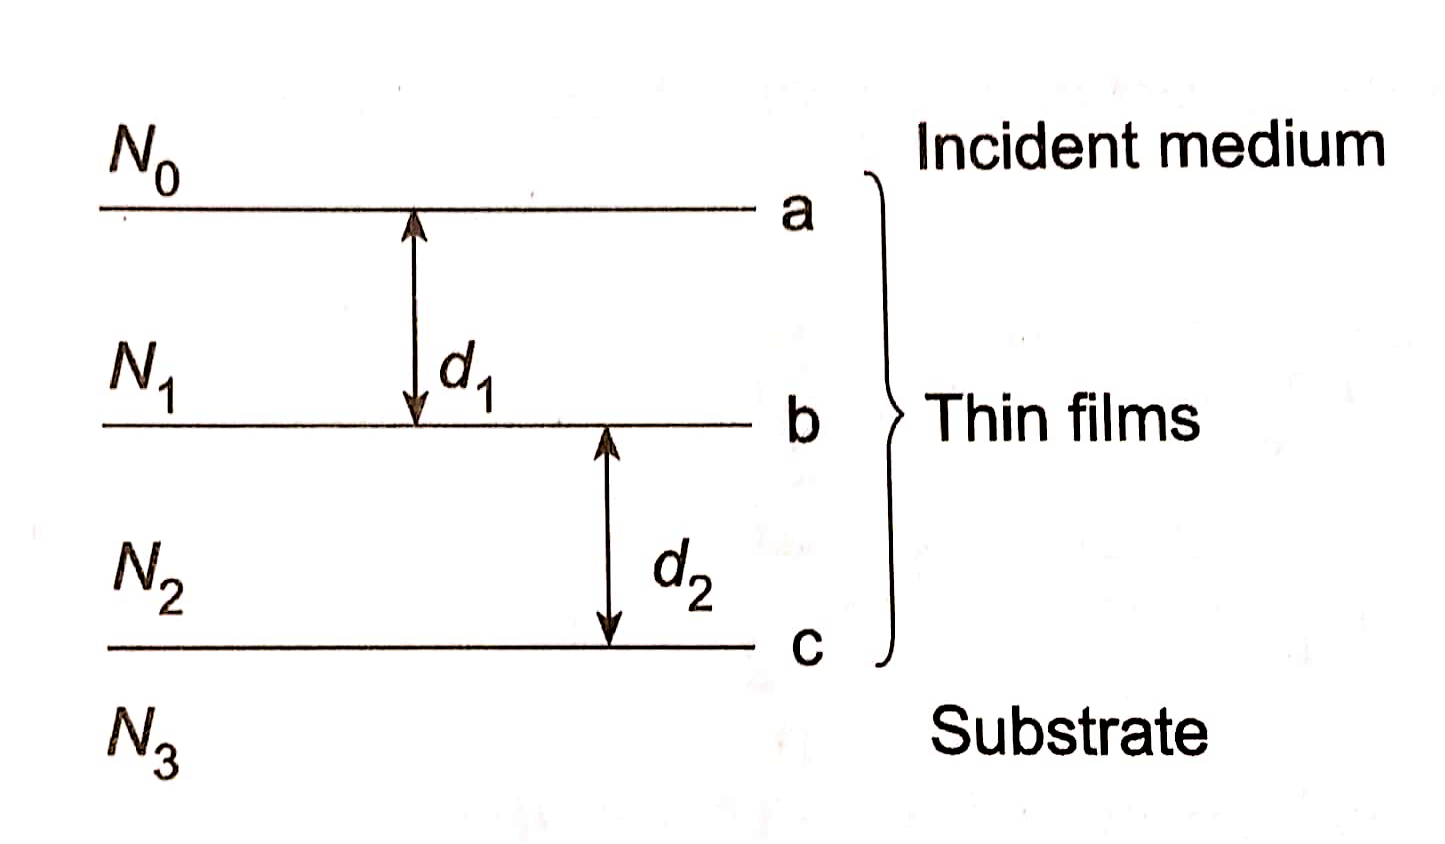
\includegraphics[width=\linewidth]{film_assembly.png}
        \caption{An assembly of thin films}
        \label{fig:assem}
    \end{figure}
    We turn our attention to the assembly found in Figure \ref{fig:assem}. By quick analogy with the previous section, is it readily seen that the characteristic matrix of the assembly is given by
    \begin{equation}
        \begin{bmatrix}
            B \\
            C
        \end{bmatrix}
        =
        \left\{\prod_{r=1}^q
        \begin{bmatrix}
            \cos \delta_r & (i \sin \delta_r)/\eta_r \\
            i \eta_r \sin \delta_r & \cos \delta_r            
        \end{bmatrix}
        \right\}
        \begin{bmatrix}
            1 \\
            \eta_m            
        \end{bmatrix}
    \end{equation}
    The admittance and reflectance of the assembly are calculated as described before in (\ref{eq:filmadmit}) and (\ref{eq:filmreflec})

\section{Transmission through a Thin Film Assembly}
    We calculate the net irradiance leaving the assembly as
    \begin{align}
        I_k &= \frac{1}{2}\Re\left(E_k H_k^*\right) \\
            &= \frac{1}{2}\Re\left(\eta_m^*\right) E_k E_k^*
    \end{align}
    If the characteristic matrix of the assembly is
    \begin{equation*}
        \begin{bmatrix}
            B \\
            C
        \end{bmatrix}        
    \end{equation*}
    The incident irradiance on the assembly is given by
    \begin{equation}
        I_a = \frac{1}{2}\Re\left(BC^*\right)E_k E_k^*        
    \end{equation}
    The transmittance is, as always, given by the ratio of incident irradiance to exit irradiance
    \begin{equation}
        T = \frac{I_k}{I_i} = \frac{\Re\left(\eta_m\right)(1-R)}{\Re\left(B C^*\right)}        
    \end{equation}
    which can be modified to
    \begin{equation}
        T = \frac{4 \eta_0 \Re(\eta_m)}{(\eta_0 B + C)(\eta_0 B + C)^*} 
    \end{equation}
    For the transmittance to have physical meaning, the incident medium must be transparent. That is, $\eta_0$ must be real

\section{Quarter and Half-Wave Thickness}
    Of considerable importance in thin film optical assemblies are layers where the optical thickness are an integer number of quarter waves. That is, if
    \begin{equation*}  
        \delta = \frac{m \pi}{2}, \text{	} m = 0, 1, 2, 3 \ldots
    \end{equation*}
    For $m$ even, the layer is an integer number of half wavelengths, and the matrix becomes
    \begin{equation*}
        \pm
        \begin{bmatrix}
            1 & 0 \\
            0 & 1                        
        \end{bmatrix}
    \end{equation*}
    This is the unity matrix, and therefore has no effect on the reflectance or transmittance of the assembly.

    For $m$ odd, the matrix becomes
    \begin{equation*}
        \pm
        \begin{bmatrix}
            0 & i/\eta \\
            i \eta & 0
        \end{bmatrix}
    \end{equation*}
    Of more importance with the quarter wavelength layer is what happens in a multilayer film consisting of high-index and low-index layers. Light reflected within the low-index layers will experience a phase-shift of $\pi$, while light reflected in the high-index layers will not experience a phase shift. Therefore, all light coming off the front surface of the multilayer will be in-phase, and the film can have an extraordinarily high reflectance for a limited range of wavelengths. This phenomenon is of extreme importance to devices discussed later.
\end{document}